\begin{mdframed}[frametitle={Change in notation}, nobreak=false]
    From this section onward, $\Omega$ (`Omega') denotes the frequency in the context of a continuous-time signal; whereas $\omega$ (`omega') denotes the frequency in the context of a discrete-time signal. \\

    Hence, the continuous-time Fourier transform (CTFT):
    \[
        \underbrace{X(\omega) = \int_{-\infty}^{+\infty} x(t) e^{-j\omega t} \mathrm{d}t}_{\text{old notation}}
        \quad \Rightarrow \quad 
        \underbrace{X(j\Omega) = \int_{-\infty}^{+\infty} x(t) e^{-j\Omega t} \mathrm{d}t}_{\text{new notation}}
    \]
\end{mdframed}


\section{Sampling}
\begin{figure}[H]
    \centering
    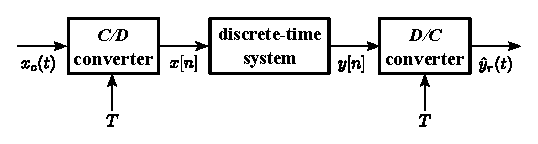
\includegraphics[width=.65\textwidth]{images/digital-processing-of-continuous-signals-short.eps}
    \caption{An (very-brief) overview of  digital processing of continuous-time signals}
    \label{fig:dsp_short}
\end{figure}
\autoref{fig:dsp_short} illustrates a concise process of digital processing of a continuous-time signal. 
\begin{itemize}
    \item The C/D conversion involves sampling a continuous-time signal to obtain a discrete-time signal.

    \item The D/C conversion involves the reconstruction of a continuous0-time signal from the sampled discrete-time signal.
\end{itemize} 

\subsection{Sampling of a Continuous-Time Signal}
Mathematically, sampling of a continuous-time signal $x_{c}(t) \to x[n]$ is:
\[ x[n] = x_{c}(nT) \quad -\infty < n < +\infty \]
where $T$ is sampling period, $f_{s} = \frac{1}{T}$ is sampling frequency (or $\Omega_{s}=\frac{2\pi}{T}$ in radians). 
\begin{itemize}
    \item In general, the C/D transformation cannot be inverted.
    \item Infinite continuous signals can reproduce a given sequence of samples,
\end{itemize}
An ideal C/D converter applies the $T$ property so that the sampling can be done without losing information. \\


Impulse train modulator $s(t)$ is: 
\[ 
    s(t) = \sum_{n=-\infty}^{+\infty} \ \delta(t-nT) 
\]
The sampled signal $x_{s}(t)$ is obtained by multiplying the impulse train modulator (\autoref{fig:original_signal}.b) with the continuous-time signal $x_{c}(t)$ of interest (\autoref{fig:original_signal}.a):
\begin{align*} 
\begin{split}
x_{s}(t) &= x_{c}(t) \ s(t)\\
&= \sum_{n=-\infty}^{+\infty} x_{c}(t) \delta(t-nT)\\
&= \sum_{n=-\infty}^{+\infty} x_{c}(nT) \delta(t-nT)
\end{split}
\end{align*}
Sampled signal, $x_{s}(t)$, is still defined in the continuous-time domain, but it contains all information in the sampled discrete-time domain.\\\\

\begin{minipage}{\textwidth}
\begin{wrapfigure}{r}{0.5\textwidth}
    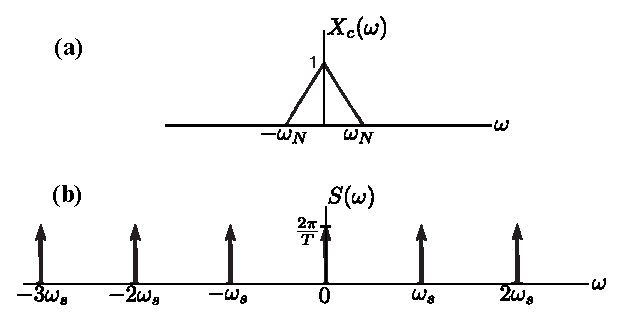
\includegraphics[width = 0.6\textwidth]{images/sample_signal_delta_train.eps}
    \caption{Spectrum of (a) the original continuous-time signal pending to be sampled; (b) sampling signal (delta train)}
    \label{fig:original_signal}
\end{wrapfigure}
Apply the Fourier transform to  $x_{s}(t)$:
\begin{align*} 
\begin{split}
    X_{s}(\Omega) 
    & = \mathcal{FT}\{x_{c}(t)\} \cdot \mathcal{FT}\{s(t)\}\\
    & = \frac{1}{2\pi} X_{c}(\Omega) * \mathcal{FT}\{s(t)\} \\
    & = \frac{1}{T} X_{c}(\Omega) * \sum_{n=-\infty}^{+\infty} \delta (\Omega - k \Omega_{s})\\
    & = \boxed{\frac{1}{T} \sum_{n=-\infty}^{+\infty}  X_{c}(\Omega - k \Omega_{s})}
\end{split} 
\end{align*}
where sampling frequency $\Omega_{s}=\Omega_{0}=\frac{2\pi}{T}$.
\end{minipage}
\ \\\\\\\\
For sampled signals: $\Omega_{N}$ is the signal bandwidth
\begin{itemize}
    \item if $\Omega_{s} \geq 2\Omega_{N}$, the replicas in the periodization do not overlap (\autoref{fig:aliasing}.a)
    \item if $\Omega_{s} < 2\Omega_{N}$, the replicas overlap, also known as \textbf{aliasing}(\autoref{fig:aliasing}.b).
\end{itemize} 

\begin{figure}[H]
    \centering
    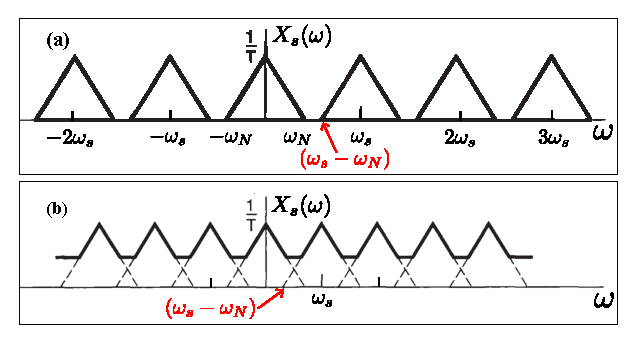
\includegraphics[width = 0.7\textwidth]{images/sampling_aliasing.eps}
    \caption{(a) Sampling without aliasing, $\omega_{s} \geq 2\omega_{N}$; \ (b) Sampling with aliasing, $\omega_{s} < 2\omega_{N}$} 
    \label{fig:aliasing}
\end{figure}



\subsubsection{Nyquist-Shannon Sampling Theorem}
Nyquist-Shannon sampling theorem states that: \textbf{to retain the ability to reproduce (reconstruct) the original signal, the minimum sampling frequency during signal sampling must be at least twice its frequency.}\\

Mathematically, let $x_{c}(t)$ be a band-limited signal with $X_{c}(\Omega)=0$, for $\lvert \Omega \rvert \geq \Omega_{N}$. Then $x_{c}(t)$ is uniquely determined by its samples $x[n] = x_{c}(nT)$, if 
\[ \Omega_{s}=\frac{2\pi}{T} \geq 2\Omega_{N} \]
where $2\Omega_{N}$ is the minimal sampling rate and referred to as the \textbf{Nyquist rate}.\\

Nyquist-Shannon sampling theorem provides the condition under which the C/D transformation \textbf{can be inverted} without losing information, as shown in \autoref{fig:nyquist}.

\begin{figure}[H]
    \centering
    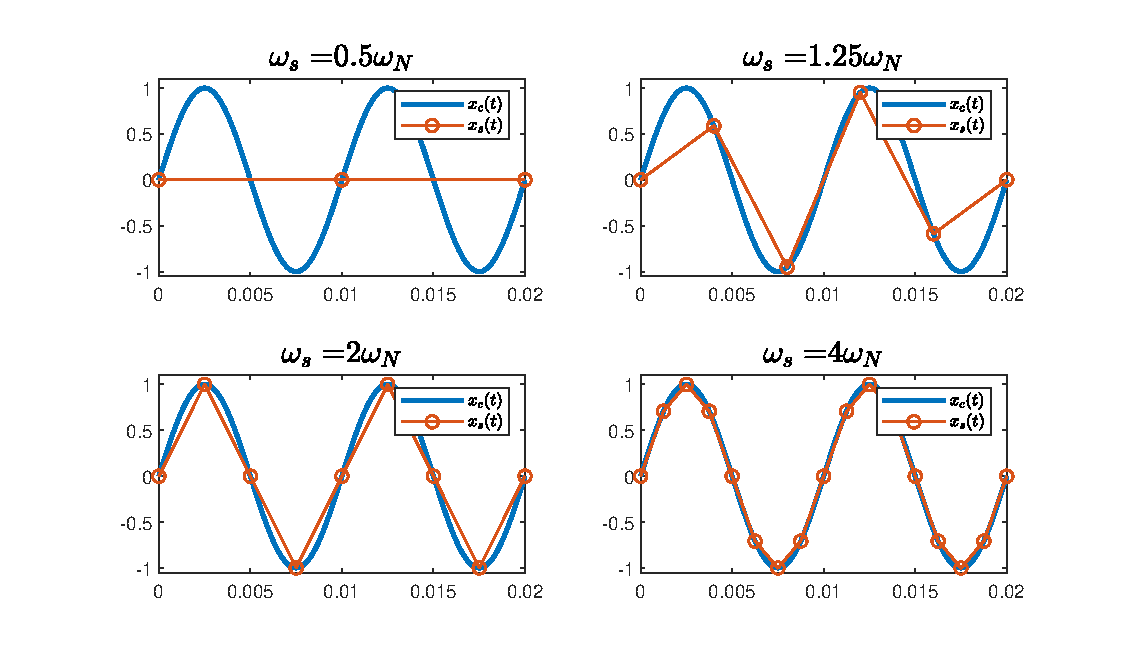
\includegraphics[width=.95\textwidth, center]{images/nyquist.eps}
    \caption{Sampling of a continuous signal $x_{c}(t)=\sin(200\pi t)$: (left to right, top to bottom) $\omega_{s}=0.5\omega_{N}$, $\omega_{s}=1.25\omega_{N}$, $\omega_{s}=2\omega_{N}$, $\omega_{s}=4\omega_{N}$. According to the Nyquist-Shannon sampling theorem, aliasing occurs when $\omega_{s} < 2\omega_{N}$}
    \label{fig:nyquist}
\end{figure}

\subsection{Practical Digital Processing of Continuous-Time Signals}
\begin{figure}[H]
    \centering
    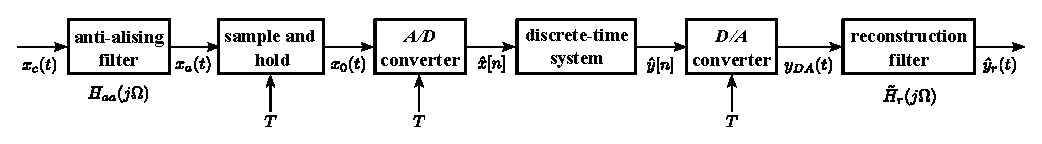
\includegraphics[width=\textwidth]{images/digital-processing-of-continuous-signals.eps}
    \caption{Overview of practical digital processing of continuous-time signals}
    \label{fig:dsp}
\end{figure}

\paragraph{Ideal anti-aliasing filter: $x_{c}(t) \to x_{a}(t)$}
\[
    H_{aa}(j\Omega) = 
    \begin{cases}
    1,  & \lvert \Omega \rvert \leq \pi/T \\
    0,  & \lvert \Omega \rvert > \pi/T
    \end{cases}
\]

\paragraph{Sample and hold: $x_{a}(t) \to x_{0}(t)$}
\[
    x_0(t) = h_0(t) * \sum_{n=-\infty}^{\infty} x_{c}(nT)\delta(t-nT)
\]

\paragraph{Practical D/A conversion: $\hat{y}[n] \to y_{DA}(t)$}
\[
    x_{c}(t) = \sum_{n=-\infty}^{+\infty} x_{c}(nT)h_{r}(t-nT) = \sum_{n=-\infty}^{+\infty} x_{c}(nT) \frac{\sin(\pi(t-nT)/T)}{\pi(t-nT)/T}
\]
\[
    x_{DA}(t) = \sum_{n=-\infty}^{+\infty} x[n]h_{p}(t-nT) + \sum_{n=-\infty}^{+\infty} e[n]h_{p}(t-nT)
\]

